\section{第二部分}
\subsection{子标题1.1}
\begin{frame}{\insertsubsection}
	\begin{columns}
		\column{0.35\textwidth}
		常见的研究方法:
		\begin{itemize}
			\item<1-> a
			\item<2-> b		
		\end{itemize}
		\column{0.65\textwidth}
		\begin{center}
			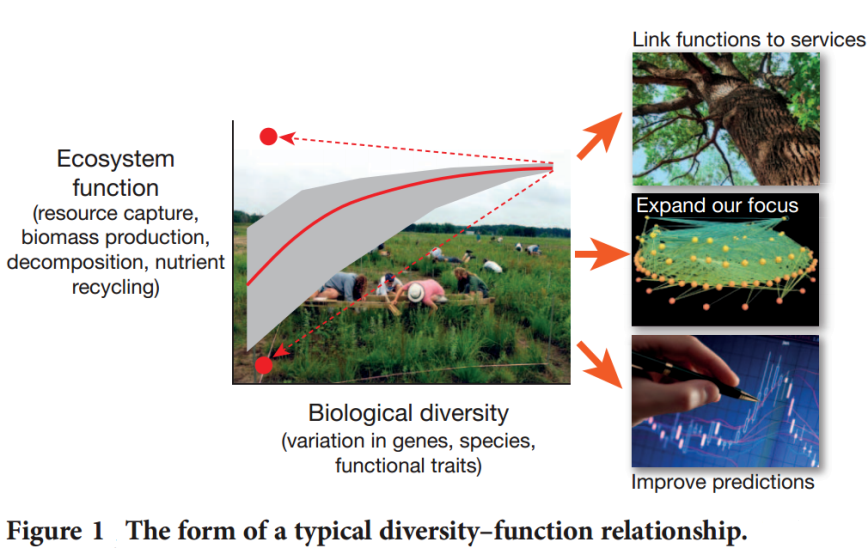
\includegraphics[width = \textwidth]{./pic/2.1.1.png}
		\end{center}
	\end{columns}
\end{frame}


\subsection{子标题2.2}
\begin{frame}{\insertsubsection}
	内容...
\end{frame}


